\documentclass{beamer}


\usepackage{amssymb,amsmath}
\usepackage{graphicx}
\usepackage{url}
\usepackage{color}
\usepackage{relsize}		% For \smaller
\usepackage{url}			% For \url
\usepackage{epstopdf}	% Included EPS files automatically converted to PDF to include with pdflatex
\usepackage{pagenote}[continuous,page]

%For MindMaps
% \usepackage{tikz}%
% \usetikzlibrary{mindmap,trees,arrows}%

%%% Color Definitions %%%%%%%%%%%%%%%%%%%%%%%%%%%%%%%%%%%%%%%%%%%%%%%%%%%%%%%%%
%\definecolor{bordercol}{RGB}{40,40,40}
%\definecolor{headercol1}{RGB}{186,215,230}
%\definecolor{headercol2}{RGB}{80,80,80}
%\definecolor{headerfontcol}{RGB}{0,0,0}
%\definecolor{boxcolor}{RGB}{186,215,230}

%%% Save space in lists. Use this after the opening of the list %%%%%%%%%%%%%%%%
%\newcommand{\compresslist}{
%	\setlength{\itemsep}{1pt}
%	\setlength{\parskip}{0pt}
%	\setlength{\parsep}{0pt}
%}

%\setbeameroption{show notes on top}

% You should run 'pdflatex' TWICE, because of TOC issues.

% Rename this file.  A common temptation for first-time slide makers
% is to name it something like ``my_talk.tex'' or
% ``john_doe_talk.tex'' or even ``discrete_math_seminar_talk.tex''.
% You really won't like any of these titles the second time you give a
% talk.  Try naming your tex file something more descriptive, like
% ``riemann_hypothesis_short_proof_talk.tex''.  Even better (in case
% you recycle 99% of a talk, but still want to change a little, and
% retain copies of each), how about
% ``riemann_hypothesis_short_proof_MIT-Colloquium.2000-01-01.tex''?

\mode<presentation>
{
  % A tip: pick a theme you like first, and THEN modify the color theme, and then add math content.
  % Warsaw is the theme selected by default in Beamer's installation sample files.

  %%%%%%%%%%%%%%%%%%%%%%%%%%%% THEME
  %\usetheme{Madrid}		% No subsection
  \usetheme{AnnArbor}  % Subsection on top, no color


  %\usetheme{Antibes}
  %\usetheme{Bergen}
  %\usetheme{Berkeley}		% bem bacana - menu esquerdo
  %\usetheme{Berlin}
  %\usetheme{Boadilla}
  %\usetheme{boxes}
  %\usetheme{CambridgeUS}		% bem bacana - menu superior
  %\usetheme{Copenhagen}
  %\usetheme{Darmstadt}
  %\usetheme{default}
  %\usetheme{Dresden}
  %\usetheme{Frankfurt}
  %\usetheme{Goettingen}
  %\usetheme{Hannover}		% bem bacana - menu esquerdo
  %\usetheme{Ilmenau}
  %\usetheme{JuanLesPins}
  %\usetheme{Luebeck}
  %\usetheme{Malmoe}
  %\usetheme{Marburg}		% bem bacana - menu direito
  %\usetheme{Montpellier}
  %\usetheme{PaloAlto}		% bem bacana - menu esquerdo
  %\usetheme{Pittsburgh}
  %\usetheme{Rochester}		%bacana
  %\usetheme{Singapore}
  %\usetheme{Szeged}
  %\usetheme{Warsaw}

  %%%%%%%%%%%%%%%%%%%%%%%%%%%% COLOR THEME
  %\usecolortheme{default}		% branco, azul clarinho
  \usecolortheme{crane}		% Very yellow (ok)

  %\usecolortheme{albatross}		% azul escuro, massa
  %\usecolortheme{beetle}		% cinza, menu azul
  %\usecolortheme{dolphin}		% azul e branco, legal
  %\usecolortheme{dove}			% cinza e branco, feio
  %\usecolortheme{fly}			% todo cinza, horrível
  %\usecolortheme{lily}			% parece o default
  %\usecolortheme{orchid}		% azul e branco, ok
  %\usecolortheme{rose}			% branco e violeta-claro, bonito
  %\usecolortheme{seagull}		% cinza, feio
  %\usecolortheme{seahorse}		% nhé, meio feio
  %\usecolortheme{sidebartab}		% Azul, branco, destaque na tab, interessante
  %\usecolortheme{structure}		% bichado
  %\usecolortheme{whale}		% Azul e branco, bem bonito

  %%%%%%%%%%%%%%%%%%%%%%%%%%%% OUTER THEME
  \useoutertheme{default}
  %\useoutertheme{infolines}
  %\useoutertheme{miniframes}
  %\useoutertheme{shadow}
  %\useoutertheme{sidebar}
  %\useoutertheme{smoothbars}
  %\useoutertheme{smoothtree}
  %\useoutertheme{split}
  %\useoutertheme{tree}

  %%%%%%%%%%%%%%%%%%%%%%%%%%%% INNER THEME
  \useinnertheme{circles}
  %\useinnertheme{default}
  %\useinnertheme{inmargin}
  %\useinnertheme{rectangles}
  %\useinnertheme{rounded}

  %%%%%%%%%%%%%%%%%%%%%%%%%%%%%%%%%%%

  \setbeamercovered{invisible} % or whatever (possibly just delete it)
  % To change behavior of \uncover from graying out to totally
  % invisible, can change \setbeamercovered to invisible instead of
  % transparent. apparently there are also 'dynamic' modes that make
  % the amount of graying depend on how long it'll take until the
  % thing is uncovered.

}


% Get rid of nav bar
\beamertemplatenavigationsymbolsempty

% Use short top
%\usepackage[headheight=12pt,footheight=12pt]{beamerthemeboxes}
%\addheadboxtemplate{\color{black}}{
%\hskip0.5cm
%\color{white}
%\insertshortauthor \ \ \ \
%\insertframenumber \ \ \ \ \ \ \
%\insertsection \ \ \ \ \ \ \ \ \ \ \ \ \ \ \ \ \  \insertsubsection
%\hskip0.5cm}
%\addheadboxtemplate{\color{black}}{
%\color{white}
%\ \ \ \
%\insertsection
%}
%\addheadboxtemplate{\color{black}}{
%\color{white}
%\ \ \ \
%\insertsubsection
%}

% Insert frame number at bottom of the page.
% \usefoottemplate{\hfil\tiny{\color{black!90}\insertframenumber}}

%% makes the ppagenote command for figure references at the end.

\usepackage[english]{babel}
%qq\usepackage[latin1]{inputenc}
\usepackage{CJKutf8}
\usepackage{subfigure}

\usepackage{times}
\usepackage[T1]{fontenc}

\makepagenote
\renewcommand{\notenumintext}[1]{}
\newcommand{\ppagenote}[1]{\pagenote[Page \insertframenumber]{#1}}

\title[Programming Challenges]{GB20602 - Programming Challenges}
\author[Claus Aranha]{Claus Aranha\\{\footnotesize caranha@cs.tsukuba.ac.jp}}
\institute[U. Tsukuba]{University of Tsukuba, Department of Computer Sciences}


\title[GB21802]{GB21802 - Programming Challenges}
\subtitle[]{Week 0 - Introduction}
\author[Claus Aranha]{Claus Aranha\\{\footnotesize caranha\@@cs.tsukuba.ac.jp}}
\institute{Department of Computer Science}

\begin{document}

\begin{frame}
\maketitle
\end{frame}


%%%%%%%
\section{Introduction}
\subsection{Course Description}

\begin{frame}
  \frametitle{What is this course about?}
  \begin{block}{A ``Strange'' Course}
    {\bf Goal}: Improve the understanding of algorithms and programming techniques.\\
    {\bf Method}: Solve short and hard problems using well known algorithms 
  \end{block}
\end{frame}

\begin{frame}
  \frametitle{Course Outline}
  \begin{center}
    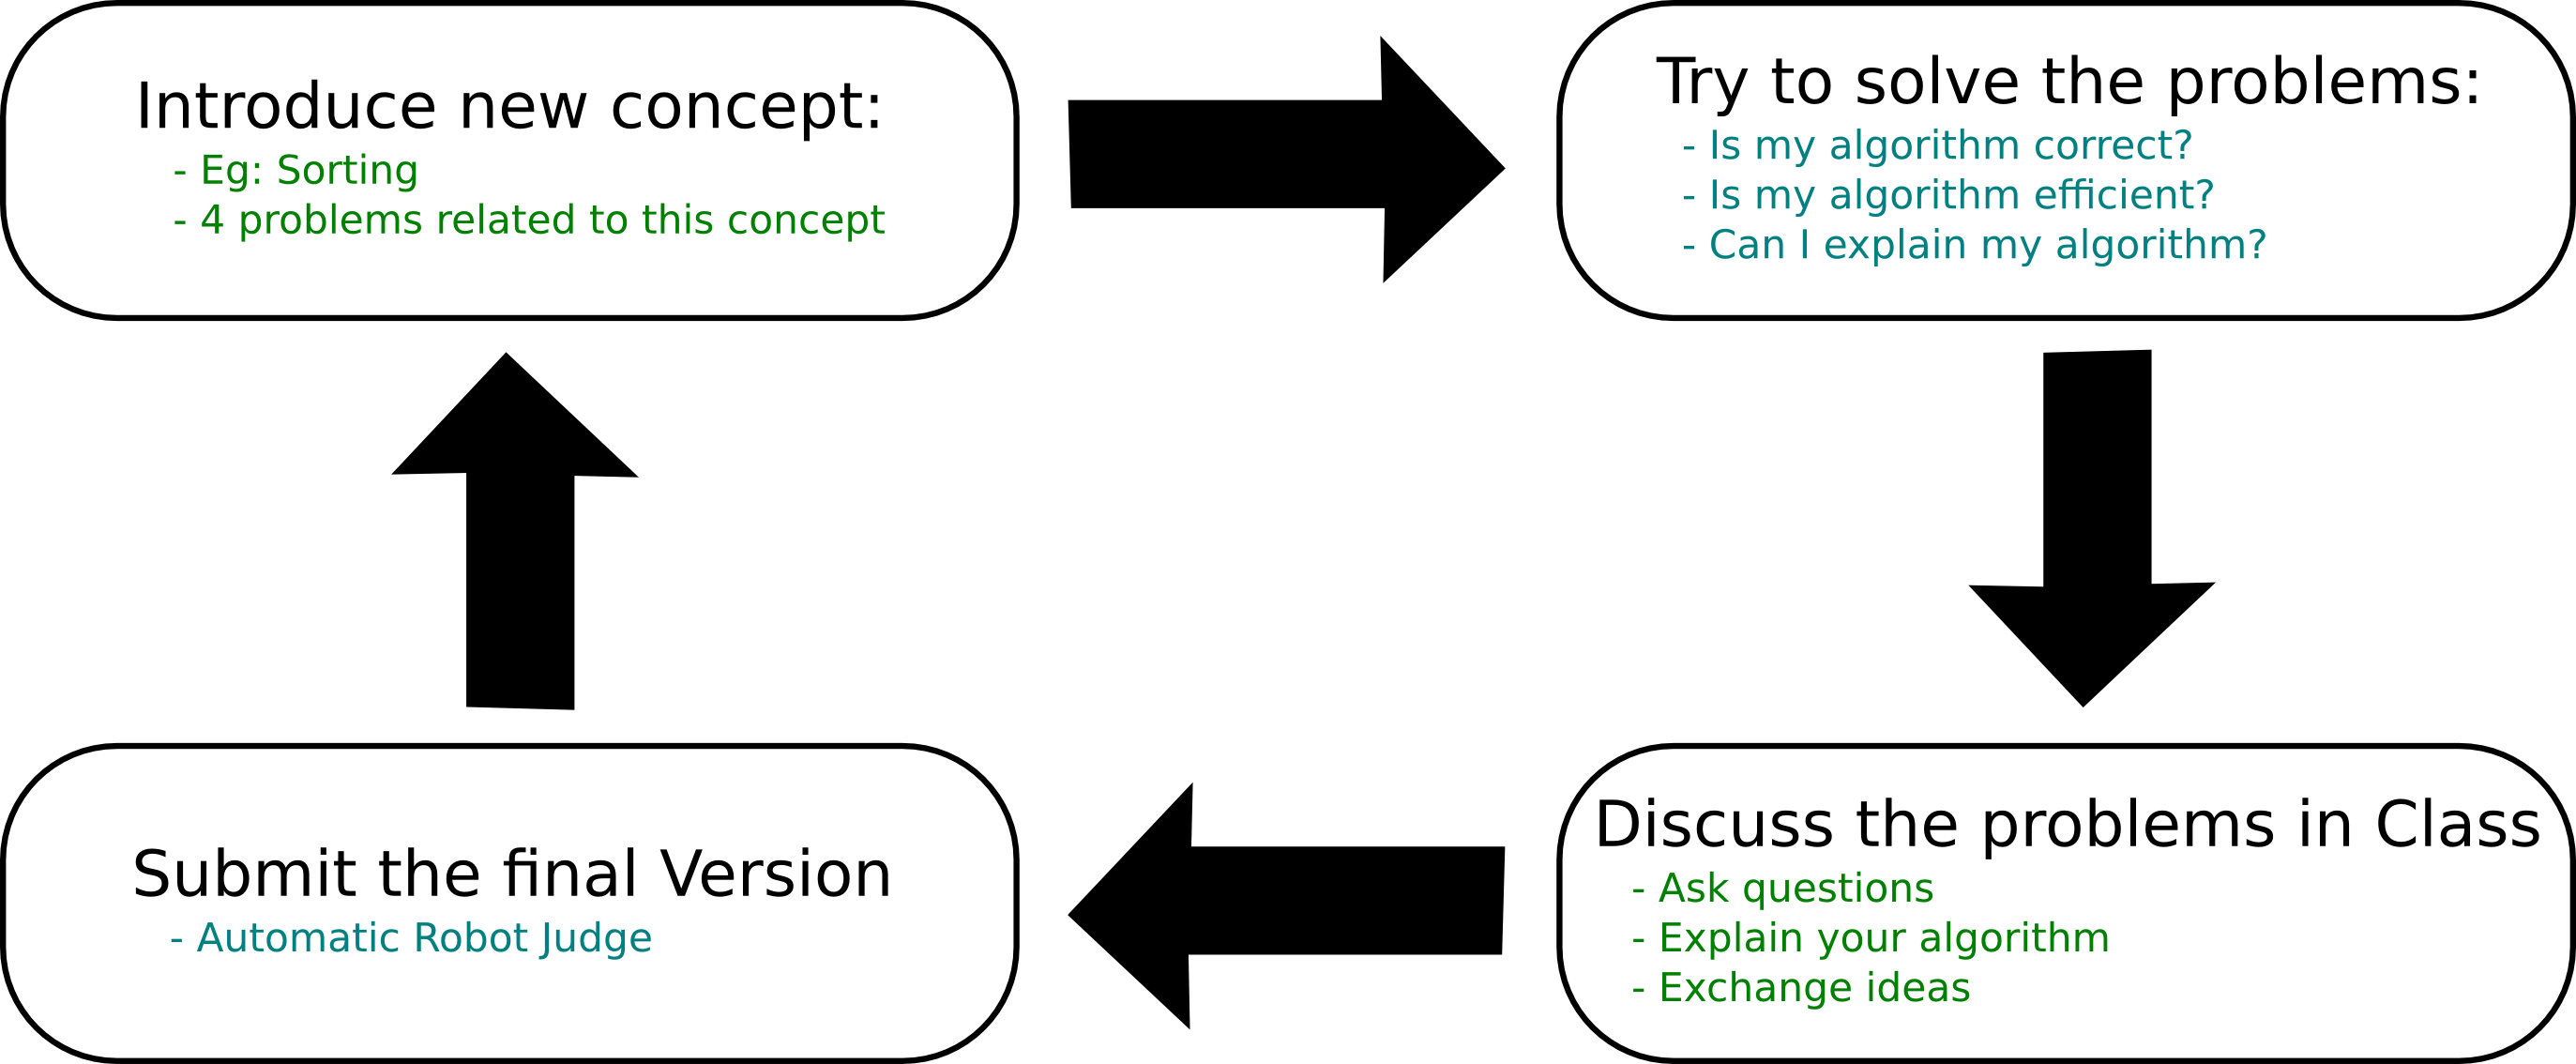
\includegraphics[width=1\textwidth]{classoutline}
  \end{center}
\end{frame}

\begin{frame}
  \frametitle{Course Languages}
  
  \begin{center}
    \begin{itemize}
    \item\structure{Program Language}: C, C++, Java, {\tiny Pascal}
    \item\structure{Spoken Language}: Japanese
    \item\structure{Materials and Problems}: English
    \item\structure{Reports and Questions}: Both!
    \end{itemize}
  \end{center}
\end{frame}

\section{Programming Challenges}
\subsection{What is a programming challenge}

\begin{frame}
  \frametitle{What are programming challenges?}
  \begin{center}
    Short (but sometimes hard) problem involving algorithms
  \end{center}

  \begin{columns}[c]
    \column{0.35\textwidth}
    \begin{block}{Components}
      \begin{itemize}
      \item \alert<1>{Problem Outline}
      \item \alert<2-3>{Example Data}
      \item \alert<2-3>{Example Result}
      \item \alert<4>{Hidden Data}
      \item \alert<5>{Judge Result}
      \end{itemize}
    \end{block}
    \column{0.65\textwidth}
    \begin{block}{}
      \begin{onlyenv}<1>
        {\small
        Start with an integer n. If n is even, divide by 2. If n is
        odd, multiply by 3 and add 1. Repeat this process with the new
        value of n, terminating when n = 1. For example:\\
        \medskip
        22 11 34 17 52 26 13 40 20 10 5 16 8 4 2 1\\
        \medskip
        In the example above, the cycle length of 22 is 16. Given any
        two numbers i and j, you are to determine the maximum cycle
        length over all numbers between i and j, including both
        endpoints.}
      \end{onlyenv}
      \begin{onlyenv}<2>
        {\small
        {\bf Input}\\        
        The input will consist of a series of pairs of integers i and
        j, one pair of integers per line. All integers will be less
        than 1,000,000 and greater than 0.\\
        \smallskip

        {\bf Output}\\
        For each pair of input integers i and j, output i, j in the
        same order in which they appeared in the input and then the
        maximum cycle length for integers between and including i and
        j.}
      \end{onlyenv}
      \begin{onlyenv}<3-4>
        {\small
        {\bf Sample Input}\\
        1 10\\
        100 200\\
        201 210\\
        900 1000\\
        
        {\bf Sample Output}\\
        1 10 20\\
        100 200 125\\
        201 210 89\\
        900 1000 174\\}
      \end{onlyenv}
      \begin{onlyenv}<5>
        Accepted\\
        Rejected\\
        Time Limited Exceeded (TLE)\\
      \end{onlyenv}
    \end{block}
  \end{columns}
\end{frame}

\section{System}
\subsection{Class Structure}
\begin{frame}
  \frametitle{How the Classes will work}
  \begin{block}{Monday}
    \structure{Problem presentation}: The week theme will be
    presented, and 4 problems regarding that theme will be shown.
  \end{block}
  \begin{block}{Friday}
    \structure{Problem discussion}: Students discuss together
    questions about problems and how to solve them.
  \end{block}
  \begin{block}{Deadline}
    Deadline for program submission is \alert{Sunday, Midnight}\\
    Programs submitted after the deadline are accepted with penalty.
  \end{block}
\end{frame}

\subsection{Evaluation}
\begin{frame}
  \frametitle{Evaluation and Grading}
  \begin{center}
    Evaluation is based on solving the programs, and participation in class.
  \end{center}
  \begin{itemize}
  \item \structure{C}: One problem per class;
  \item \structure{B}: Two problems per class, or 20 problems;
  \item \structure{A}: Three problems per class, or 30 problems;
  \end{itemize}
  \medskip
  \begin{block}{Bonus: Grade Up}
    Good participation in class and good Comments in code.
  \end{block}
  \begin{block}{Penalty: Grade Down}
    More than 25\% late problems.
  \end{block}
\end{frame}

\section{Solving Problems}
\subsection{How to submit problems}
\begin{frame}
  \frametitle{How to submit problems - 1}

  \begin{block}{Problem Submission System}
    \begin{enumerate}
      \item Make an account at \url{http://www.programming-challenges.com};\\ 
        {\small (If possible use your Student Number as ID)}
      \item Send your ID to the professor by e-mail;\\
        {\small \url{mailto:caranha@cs.tsukuba.ac.jp}}
      \item You will be added to the classroom
        \structure{Tsukuba~Programming~Challenges~2015};        
    \end{enumerate}
  \end{block}
\end{frame}

\begin{frame}
  \frametitle{How to submit problems - 2}

  \begin{block}{Problem Submission System}
    \begin{enumerate}
      \setcounter{enumi}{3}
      \item Click ``Joined Classrooms'', select
        \structure{Tsukuba~Programming~Challenges~2015};
      \item Click the name of the problem for a description, then ``Submit'' to send your code.
      \item Choose the language; upload a file or paste your code.
      \item Wait for the response from the Judge!
    \end{enumerate}
  \end{block}
\end{frame}

\begin{frame}
  \frametitle{Some notes about program submission}
  Please Keep in Mind:
  \medskip
  \begin{itemize}
  \item Don't copy programs from the internet, or from your friends;
  \item It is okay to copy \underline{ideas} from the internet or your friends;\\
    {\small If you do, mention it in the comments}
  \item Add some commentary on top of the program, explaining what you
    did, what went right, or what went wrong.    
  \end{itemize}
\end{frame}

\begin{frame}[simple,fragile]
  \frametitle{Some notes about program submission}
  \begin{block}{Good Comment}
{\small
\begin{verbatim}
/**
 * I used quicksort to solve this problem. 
 * I sorted the age of the persons in the input.
 * To make it faster, people with the same age were 
 * removed from the data.
 */
\end{verbatim}}
  \end{block}
  \begin{block}{Bad Comment}
{\small
\begin{verbatim}
/**
 * Quicksort.
 */
\end{verbatim}}
  \end{block}
\end{frame}

\begin{frame}
  \frametitle{How the Judge Works}
  \begin{block}{Accepted}
    Congratulations!
  \end{block}
  \begin{block}{\alert{Wrong Answer}}
    Your answer does not match with the judge's answer. Remember to
    check for worst-case scenarios!
  \end{block}
  \begin{block}{\alert{Time Limited Exceeded}}
    Your algorithm is too slow. Think about computational efficiency.
  \end{block}
  \begin{block}{}
    Compilation Error, Runtime Error, etc.
  \end{block}
  % Accepted, Rejected, TLE, Presentation Error
\end{frame}

\section{Extra Content}

\subsection{What are programming contests}
\begin{frame}
  \frametitle{OMAKE I: Programming Contests}

  \begin{itemize}
    \item What are Programming Contests?
    \item Examples: ACM-ICPC, TOPCODER, ATCODER, \ldots
  \end{itemize}
\end{frame}

\subsection{Introductory problems}
\begin{frame}
  \frametitle{OMAKE II: Next week's problems}
  \begin{itemize}
  \item 3n+1 Problem
  \item Minesweeper
  \item The Trip
  \item Interpreter
  \end{itemize}
  
  \begin{block}{}
    A proper introduction to these problems will be made next week!
  \end{block}

\end{frame}

\end{document}
